\documentclass[11pt, hidelinks, twoside]{article}

\usepackage{setspace}
\usepackage[headheight = 13.6pt]{geometry}
 \geometry{a4paper, total={170mm,257mm}, left=20mm, top=20mm}
\usepackage{amssymb,amsfonts,bezier,amstext,amsthm,amsmath,graphicx,makeidx,caption,subfigure,mathtools}

% --- Language Setup (English) ---
\usepackage[english]{babel} 
\usepackage[colorinlistoftodos]{todonotes}
\usepackage{bm}
\usepackage{stackengine}
\newcommand{\pr}{\hspace*{15mm}}
\newcommand{\n}{\noindent}
\newcommand{\questionequal}{\mathrel{\stackon[0.5pt]{=}{?}}}
\usepackage{lipsum}
\usepackage{textcomp}
\usepackage{gensymb}
\usepackage{mathrsfs}
\usepackage{tikz}
% \usepackage{fontspec}
\usepackage{authblk}
\usepackage{blindtext}
\usepackage{booktabs}
\usepackage[T1]{fontenc}
\usepackage{graphicx}
\graphicspath{ {./images/} }
\usepackage{amsmath}
\usepackage[bookmarksnumbered=true]{hyperref}
\usepackage{indentfirst}
\usepackage{float}
\usepackage{color}  
\usepackage{chemfig,chemmacros} 
\usepackage{pdfpages}
\usepackage{makeidx}
\usepackage{lastpage}
\usepackage{lmodern}
\usepackage{mathtools}
\usepackage{bm}
\usepackage{esvect}

% --- Custom English Labels ---
\def\figureautorefname{Figure}
\def\equationautorefname{Equation}
\def\tableautorefname{Table}

\usepackage{comment}
\usepackage{url}
\usepackage{pgfplots}
\pgfplotsset{compat=newest}
\pgfplotsset{plot coordinates/math parser=false}
\newlength\figureheight
\newlength\figurewidth
\usepackage[title]{appendix}
\usepackage{float}
\usepackage{placeins}
\usepackage{multirow}
\usepackage{hyperref}
\usepackage{tikz,tkz-euclide}
\usepackage{circuitikz}
\usepackage[framed,numbered,autolinebreaks,useliterate]{mcode}
\usepackage{verbatim}
\usepackage{fancyhdr}
\usepackage{adjustbox}
\usepackage{hyperref}
\usepackage{silence}
\usepackage{physics}
\usepackage{cancel}
\usepackage{xparse}
\usepackage{esint}
\usepackage{tikz-3dplot}
\WarningFilter{latex}{`h' float specifier changed to `ht'}

\usetikzlibrary{external}
\tikzexternalize

\hypersetup{colorlinks = true,
            linkcolor = black,
            urlcolor  = blue}

\renewcommand\lstlistingname{Code}
\setlength{\parskip}{0.2\baselineskip}

% Centered Contents Title
\addto\captionsenglish{\renewcommand{\contentsname}{\centering Contents}}

\AtBeginDocument{\RenewCommandCopy\qty\SI}
\ExplSyntaxOn
    \msg_redirect_name:nnn { siunitx } { physics-pkg } { none }
\ExplSyntaxOff

\usetikzlibrary{arrows.meta}

% --- Theorems and Corollaries in English ---
\renewcommand\qedsymbol{$\blacksquare$}
\newtheorem{theorem}{Theorem}[]
\newtheorem{corollary}{Corollary}[theorem]

% --- Sectioning depth ---
\setcounter{secnumdepth}{5}
\setcounter{tocdepth}{5}

\makeatletter
\newcommand\subsubsubsection{\@startsection{paragraph}{4}{\z@}{-2.5ex\@plus -1ex \@minus -.25ex}{1.25ex \@plus .25ex}{\normalfont\normalsize\bfseries}}
\newcommand\subsubsubsubsection{\@startsection{subparagraph}{5}{\z@}{-2.5ex\@plus -1ex \@minus -.25ex}{1.25ex \@plus .25ex}{\normalfont\normalsize\bfseries}}
\makeatother

% --- Circled elements in equations ---
\makeatletter
\newcommand\mathcircled[1]{%
  \mathpalette\@mathcircled{#1}%
}
\newcommand\@mathcircled[2]{%
  \tikz[baseline=(math.base)] \node[draw,circle,inner sep=1pt] (math) {$\m@th#1#2$};%
}
\makeatother

\makeatletter
\newcommand\mathdashedcircled[1]{%
  \mathpalette\@mathdashedcircled{#1}%
}
\newcommand\@mathdashedcircled[2]{%
  \tikz[baseline=(math.base)] \node[draw,circle,dashed,inner sep=1pt] (math) {$\m@th#1#2$};%
}
\makeatother

\numberwithin{equation}{section}

\begin{document}
\thispagestyle{empty}

\begin{figure}[ht]
    \centering
    % Ensure this path is correct in your folder
    
\includegraphics[width=8cm]{Images/ecole_centrale_lille_logo.png}
    \hfill \\[0.25cm]
\end{figure}
    
\begin{center}
    {\Large $\mathrm{e}^{-}\vec{X}$Spice} \\[0.3cm]
    \vspace{4.35cm}
    {\LARGE \textbf{Electronics for Biomedical Engineering}} \\[1cm]
    {\LARGE \textbf{Mathematical Formulation}} \\[2cm]

    \begin{flushright}
    \vspace{1.5cm}
    {\Large Gabriel SILVA}\\ [0.85cm]
    \end{flushright}
    {\large \textbf{Villeneuve-d'Ascq\\[0.2cm] 2026}}
\end{center}

\clearpage
\thispagestyle{empty}

\clearpage
\listoffigures

\clearpage
\thispagestyle{empty}

\clearpage
\tableofcontents

\clearpage

\pagestyle{fancy}
\fancyhf{}
\fancyhead[RE,RO]{$\mathrm{e}^{-}\vec{X}$Spice}
\fancyhead[LE,LO]{Mathematical Formulation}
\fancyfoot[CE,CO]{\thepage}

\addcontentsline{toc}{section}{Introduction} 

% Make sure to translate the content inside these .tex files!
%\section{Introduction}


\subsection{Business Context}

 
%\clearpage

\setcounter{page}{6}
\section{A: Opamps }
\label{sec:chap_1}
\subsection{Part 1: Theory}


\begin{spacing}{1.25}


\end{spacing}




\clearpage
\section{B: Instrumentation Amplifiers}
\label{sec:chap_2}

\subsection{Part 1: Theory}

\begin{spacing}{1.25}



\begin{figure}[htbp]
    \centering
    \tikzset{external/export next=false}
    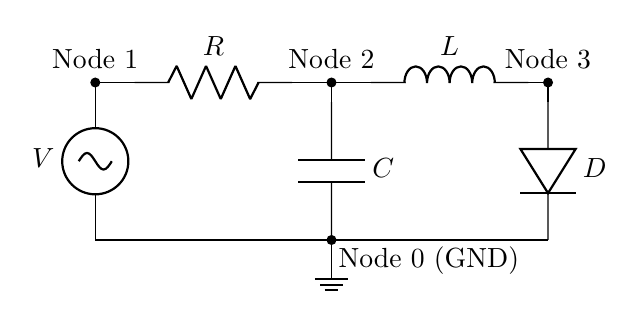
\begin{tikzpicture}[transform shape]
        % Paths, nodes and wires:
	\node[tlground] at (6.25, 4.5){};
	\draw (3.25, 6.5) to[sinusoidal voltage source, l_={$V$}] (3.25, 5.5);
	\draw (3.75, 7) to[american resistor, l={$R$}] (5.75, 7);
	\draw (6.25, 6.75) to[capacitor, l={$C$}] (6.25, 5);
	\draw (6.75, 7) to[american inductor, l={$L$}] (8.75, 7);
	\draw (9, 6.75) to[empty diode, l={$D$}] (9, 5);
	\draw (9, 5) -- (6.25, 5);
	\draw (6.25, 5) -| (6.25, 4.75);
	\draw (6.75, 7) -- (5.75, 7);
	\draw (6.25, 7) -| (6.25, 6.75);
	\draw (8.75, 7) -- (9, 7) -| (9, 6.75);
	\draw (6.25, 5) -- (3.25, 5) -| (3.25, 5.5);
	\draw (3.75, 7) -- (3.25, 7) -| (3.25, 6.5);
	\node[circ](N1) at (6.25, 7){} node[anchor=south] at (N1.north){$\text{Node 2}$};
	\node[circ](N2) at (6.25, 5){} node[anchor=north west] at ([xshift=-0.09cm, yshift=0.09cm]N2.south east){$\text{Node 0 (GND)}$};
	\node[circ](N3) at (3.25, 7){} node[anchor=south] at (N3.north){$\text{Node 1}$};
	\node[circ](N4) at (9, 7){} node[anchor=south] at (N4.north){$\text{Node 3}$};
	\draw (6.25, 4.75) -| (6.25, 4.5);
    \end{tikzpicture}
    \tikzexternalenable
    \caption{Diagrama esquemático do circuito com fonte AC, resistor, capacitor, indutor e diodo.}
    \label{fig:meu_circuito}
\end{figure}

\begin{figure}[htbp]
    \centering
    \tikzset{external/export next=false}
    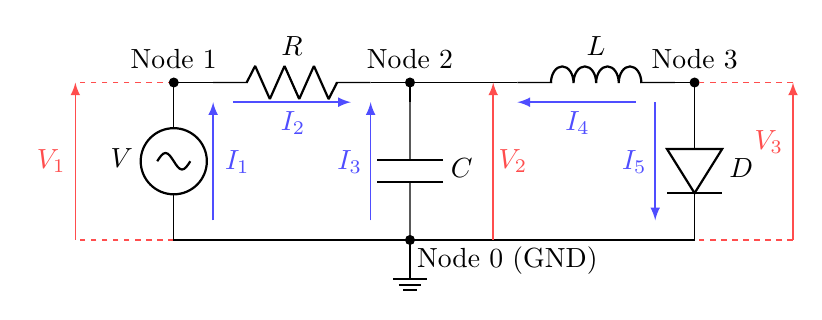
\begin{tikzpicture}[transform shape]
        % Paths, nodes and wires:
        \path[draw={rgb,255:red,255;green,77;blue,77}, line width=0.5pt, dash pattern={on 2pt off 2pt}] (3.25, 5) -- (2, 5);
        \path[draw={rgb,255:red,255;green,77;blue,77}, line width=0.5pt, dash pattern={on 2pt off 2pt}] (3.25, 7) -- (2, 7);
        \node[tlground] at (6.25, 4.5){};
        \draw (3.25, 6.5) to[sinusoidal voltage source, l_={$V$}] (3.25, 5.5);
        \draw (3.75, 7) to[american resistor, l={$R$}] (5.75, 7);
        \draw (6.25, 6.75) to[capacitor, l={$C$}] (6.25, 5);
        \draw (7.614, 7) to[american inductor, l={$L$}] (9.614, 7);
        \draw (9.864, 6.75) to[empty diode, l={$D$}] (9.864, 5);
        \draw (9.864, 5) -- (6.25, 5);
        \draw (6.25, 5) -| (6.25, 4.75);
        \draw (7.614, 7) |- (5.75, 7);
        \draw (6.25, 7) -| (6.25, 6.75);
        \draw (9.614, 7) -- (9.864, 7) -| (9.864, 6.75);
        \draw (6.25, 5) -- (3.25, 5) -| (3.25, 5.5);
        \draw (3.75, 7) -- (3.25, 7) -| (3.25, 6.5);
        \node[circ](N1) at (6.25, 7){} node[anchor=south] at (N1.north){$\text{Node 2}$};
        \node[circ](N2) at (6.25, 5){} node[anchor=north west] at ([xshift=-0.09cm, yshift=0.09cm]N2.south east){$\text{Node 0 (GND)}$};
        \node[circ](N3) at (3.25, 7){} node[anchor=south] at (N3.north){$\text{Node 1}$};
        \node[circ](N4) at (9.864, 7){} node[anchor=south] at (N4.north){$\text{Node 3}$};
        \draw (6.25, 4.75) -| (6.25, 4.5);
        
        \path[draw={rgb,255:red,79;green,77;blue,255}, line width=0.6pt, -latex] (3.75, 5.25) -- (3.75, 6.75);
        \path[draw={rgb,255:red,79;green,77;blue,255}, line width=0.6pt, -latex] (4, 6.75) -- (5.5, 6.75);
        \node[shape=rectangle, minimum width=0.351cm, minimum height=0.449cm](N5) at (4.057, 5.992){} node[anchor=center] at (N5.text){\textcolor{rgb,255:red,79;green,77;blue,255}{$I_1$}} node[anchor=north west, align=left, text width=-0.037cm, inner sep=6pt] at (3.864, 6.234){};
        \node[shape=rectangle, minimum width=0.436cm, minimum height=0.494cm](N6) at (4.765, 6.485){} node[anchor=center] at (N6.text){\textcolor{rgb,255:red,79;green,77;blue,255}{$I_2$}} node[anchor=north west, align=left, text width=0.047cm, inner sep=6pt] at (4.529, 6.75){};
        \path[draw={rgb,255:red,79;green,77;blue,255}, line width=0.6pt, -latex] (5.75, 5.25) -- (5.75, 6.75);
        \node[shape=rectangle, minimum width=0.436cm, minimum height=0.494cm](N7) at (5.485, 5.985){} node[anchor=center] at (N7.text){\textcolor{rgb,255:red,79;green,77;blue,255}{$I_3$}} node[anchor=north west, align=left, text width=0.047cm, inner sep=6pt] at (5.25, 6.25){};
        
        \path[draw={rgb,255:red,79;green,77;blue,255}, line width=0.6pt, -latex] (9.114, 6.75) -- (7.614, 6.75);
        \node[shape=rectangle, minimum width=0.436cm, minimum height=0.494cm](N8) at (8.378, 6.485){} node[anchor=center] at (N8.text){\textcolor{rgb,255:red,79;green,77;blue,255}{$I_4$}} node[anchor=north west, align=left, text width=0.047cm, inner sep=6pt] at (8.143, 6.75){};
        \path[draw={rgb,255:red,79;green,77;blue,255}, line width=0.6pt, -latex] (9.364, 6.75) -- (9.364, 5.25);
        \node[shape=rectangle, minimum width=0.436cm, minimum height=0.494cm](N9) at (9.099, 5.985){} node[anchor=center] at (N9.text){\textcolor{rgb,255:red,79;green,77;blue,255}{$I_5$}} node[anchor=north west, align=left, text width=0.047cm, inner sep=6pt] at (8.864, 6.25){};
        
        \path[draw={rgb,255:red,255;green,77;blue,77}, line width=0.6pt, -latex] (2, 5) -- (2, 7);
        \node[shape=rectangle, minimum width=0.351cm, minimum height=0.449cm](N10) at (1.693, 6.008){} node[anchor=center] at (N10.text){\textcolor{rgb,255:red,255;green,77;blue,77}{$V_1$}} node[anchor=north west, align=left, text width=-0.037cm, inner sep=6pt] at (1.5, 6.25){};
        \path[draw={rgb,255:red,255;green,77;blue,77}, line width=0.5pt, dash pattern={on 2pt off 2pt}] (11.114, 5) -- (9.864, 5);
        \path[draw={rgb,255:red,255;green,77;blue,77}, line width=0.5pt, dash pattern={on 2pt off 2pt}] (11.114, 7) -- (9.864, 7);
        \path[draw={rgb,255:red,255;green,77;blue,77}, line width=0.6pt, -latex] (11.114, 5) -- (11.114, 7);
        \node[shape=rectangle, minimum width=0.351cm, minimum height=0.449cm](N11) at (10.807, 6.242){} node[anchor=center] at (N11.text){\textcolor{rgb,255:red,255;green,77;blue,77}{$V_3$}} node[anchor=north west, align=left, text width=-0.037cm, inner sep=6pt] at (10.614, 6.484){};
        \path[draw={rgb,255:red,255;green,77;blue,77}, line width=0.6pt, -latex] (7.307, 5) -- (7.307, 7);
        \node[shape=rectangle, minimum width=0.351cm, minimum height=0.449cm](N12) at (7.557, 6.008){} node[anchor=center] at (N12.text){\textcolor{rgb,255:red,255;green,77;blue,77}{$V_2$}} node[anchor=north west, align=left, text width=-0.037cm, inner sep=6pt] at (7.364, 6.25){};
    \end{tikzpicture}
    \tikzexternalenable
    \caption{Diagrama esquemático do circuito com fonte AC, resistor, capacitor, indutor e diodo.}
    \label{fig:meu_circuito}
\end{figure}


\textbf{KCL at Node 1:}

\begin{gather*}
    I_1 - I_2 = 0 \\
    i_{V} - \frac{V_{1} - V_{2}}{R} = 0 \\
    i_{V} - (V_{1} - V_{2})G = 0
\end{gather*}

\textbf{KCL at Node 2:}
\begin{gather*}
    I_2 + I_3 + I_4 = 0 \\
    \frac{V_{1} - V_{2}}{R} + i_{C} + i_{L} = 0 \\
    \frac{V_{1} - V_{2}}{R} + (- C\frac{dV_{2}}{dt}) + i_{L} = 0 \\
    (V_{1} - V_{2})G + (- C\frac{dV_{2}}{dt}) + i_{L} = 0
\end{gather*}

\textbf{KCL at Node 3:}

\begin{gather*}
    -I_4 - I_5 = 0 \\
    i_{L} - i_{D} = 0 \\
    i_{D} - I_s \left( e^{\frac{e_3}{V_T}} - 1 \right) = 0
\end{gather*}

\textbf{KVL}







\end{spacing}

%\clearpage
%\begin{thebibliography}{9}

\bibitem{Notas de Aula}
MARTINS, Emiliano Rezende. \textbf{Mecânica Quântica para Engenharia I e II}. Curso de Engenharia Elétrica. Notas de Aula. Universidade de São Paulo.

\bibitem[Cohen, 2020]{Cohen}
COHEN-TANNOUDJI, Claude; DIU, Bernard; LALOË, Frank. \textbf{Quantum Mechanics}: Volume I: Basic Concepts, Tools, and Applications. 2. ed. Germany: Wiley-VCH, 2020. 131 - 136 p. v. 1. ISBN 978-3-527-82270-6.

\bibitem[Griffiths, 1999]{Griffiths ED 3ed}
GRIFFITHS, David J. \textbf{Introduction to Electrodynamics}. 3. ed. Upper Saddle River, New Jersey 07458, USA: Prentice-Hall Inc. ISBN 0-13-805326-X. Disponível em: \url{https://drive.uqu.edu.sa/_/quc_physics/files/Electromagnetics_by_Griffiths-1.pdf}.

\bibitem[McCoy, 1929]{McCoy1929}
MCCOY, Neal H. On commutation formulas in the algebra of quantum mechanics. \textbf{Transactions of the American Mathematical Society}, Providence, v. 31, n. 4, p. 793--806, out. 1929. DOI: 10.1090/S0002-9947-1929-1501512-1. Disponível em: \url{https://scispace.com/pdf/on-commutation-formulas-in-the-algebra-of-quantum-mechanics-39t7lv37sk.pdf}.

\end{thebibliography}

\addcontentsline{toc}{section}{Referências}

% https://www.todamateria.com.br/referencias-abnt/ (Gerador Automático de Referência)

\end{document}